\begin{frame}[label=background]{Structure Background}
    \frametitle{Structure}
    \begin{itemize}
        \item Research Questions
        \item {\color{tud grapefruit}Mathematical Background}
        \item Related Work
        \item Preliminary Results
        \item Outlook
    \end{itemize}
\end{frame}

\footerinfootnotestrue
\begin{frame}[label=background,fragile]{Background: CG method}
    \frametitle{Mathematical Background}
    \framesubtitle{Conjugate gradient method}
    \begin{algorithm}[H]
        \begin{algorithmic}
            \State $\mathbf{r}_0 = \mathbf{b} - A\mathbf{u}_0$, $\mathbf{p}_0 = \mathbf{r}_0$, $\beta_0 = 0$
            \For{$j = 0, 1, 2, \dots, m$}
            \State $\alpha_j = (\mathbf{r}_j, \mathbf{r}_j) / (A \mathbf{p}_j, \mathbf{p}_j)$
            \State $\mathbf{u}_{j+1} = \mathbf{u}_j + \alpha_j \mathbf{p}_j$
            \State $\mathbf{r}_{j+1} = \mathbf{r}_j - \alpha_j A \mathbf{p}_j$
            \State $\beta_j = (\mathbf{r}_{j+1}, \mathbf{r}_{j+1}) / (\mathbf{r}_j, \mathbf{r}_j)$
            \State $\mathbf{p}_{j+1} = \mathbf{r}_{j+1} + \beta_j \mathbf{p}_j$
            \EndFor
        \end{algorithmic}
        \caption{Conjugate Gradient Method \cite{iter_method_saad}}
    \end{algorithm}
\end{frame}

\footerinfootnotesfalse
\begin{frame}[label=background,fragile]{Background: CG explained}
    \frametitle{Mathematical Background}
    \framesubtitle{Conjugate gradient method}
    \begin{columns}[T,onlytextwidth]
        \begin{column}{.5\textwidth}
            \begin{itemize}
                \item<+-> Iterative, projection method onto a Krylov subspace $\mathcal{K}_m(A_0, \mathbf{r}_0)$ given by
                \begin{equation*}
                     \text{span}\{\mathbf{r}_0, A\mathbf{r}_0, A^2\mathbf{r}_0, \dots, A^{m-1}\mathbf{r}_0\}
                \end{equation*}
                \item<+-> Approximate solution can be expressed as
                \begin{equation*}
                    \mathbf{u}_m = \mathbf{u}_0 + \sum_{i=0}^{m-1} c_i A^i \mathbf{r}_0 = \mathbf{u}_0 + \alert<3>{q_{m-1}}(A)\mathbf{r}_0
                \end{equation*}
                \item<4> Minimize residual polynomial on eigenvalues of $A$
            \end{itemize}
        \end{column}
        \begin{column}{.5\textwidth}
            \only<3-4>{%
                \begin{figure}
                    \centering
                    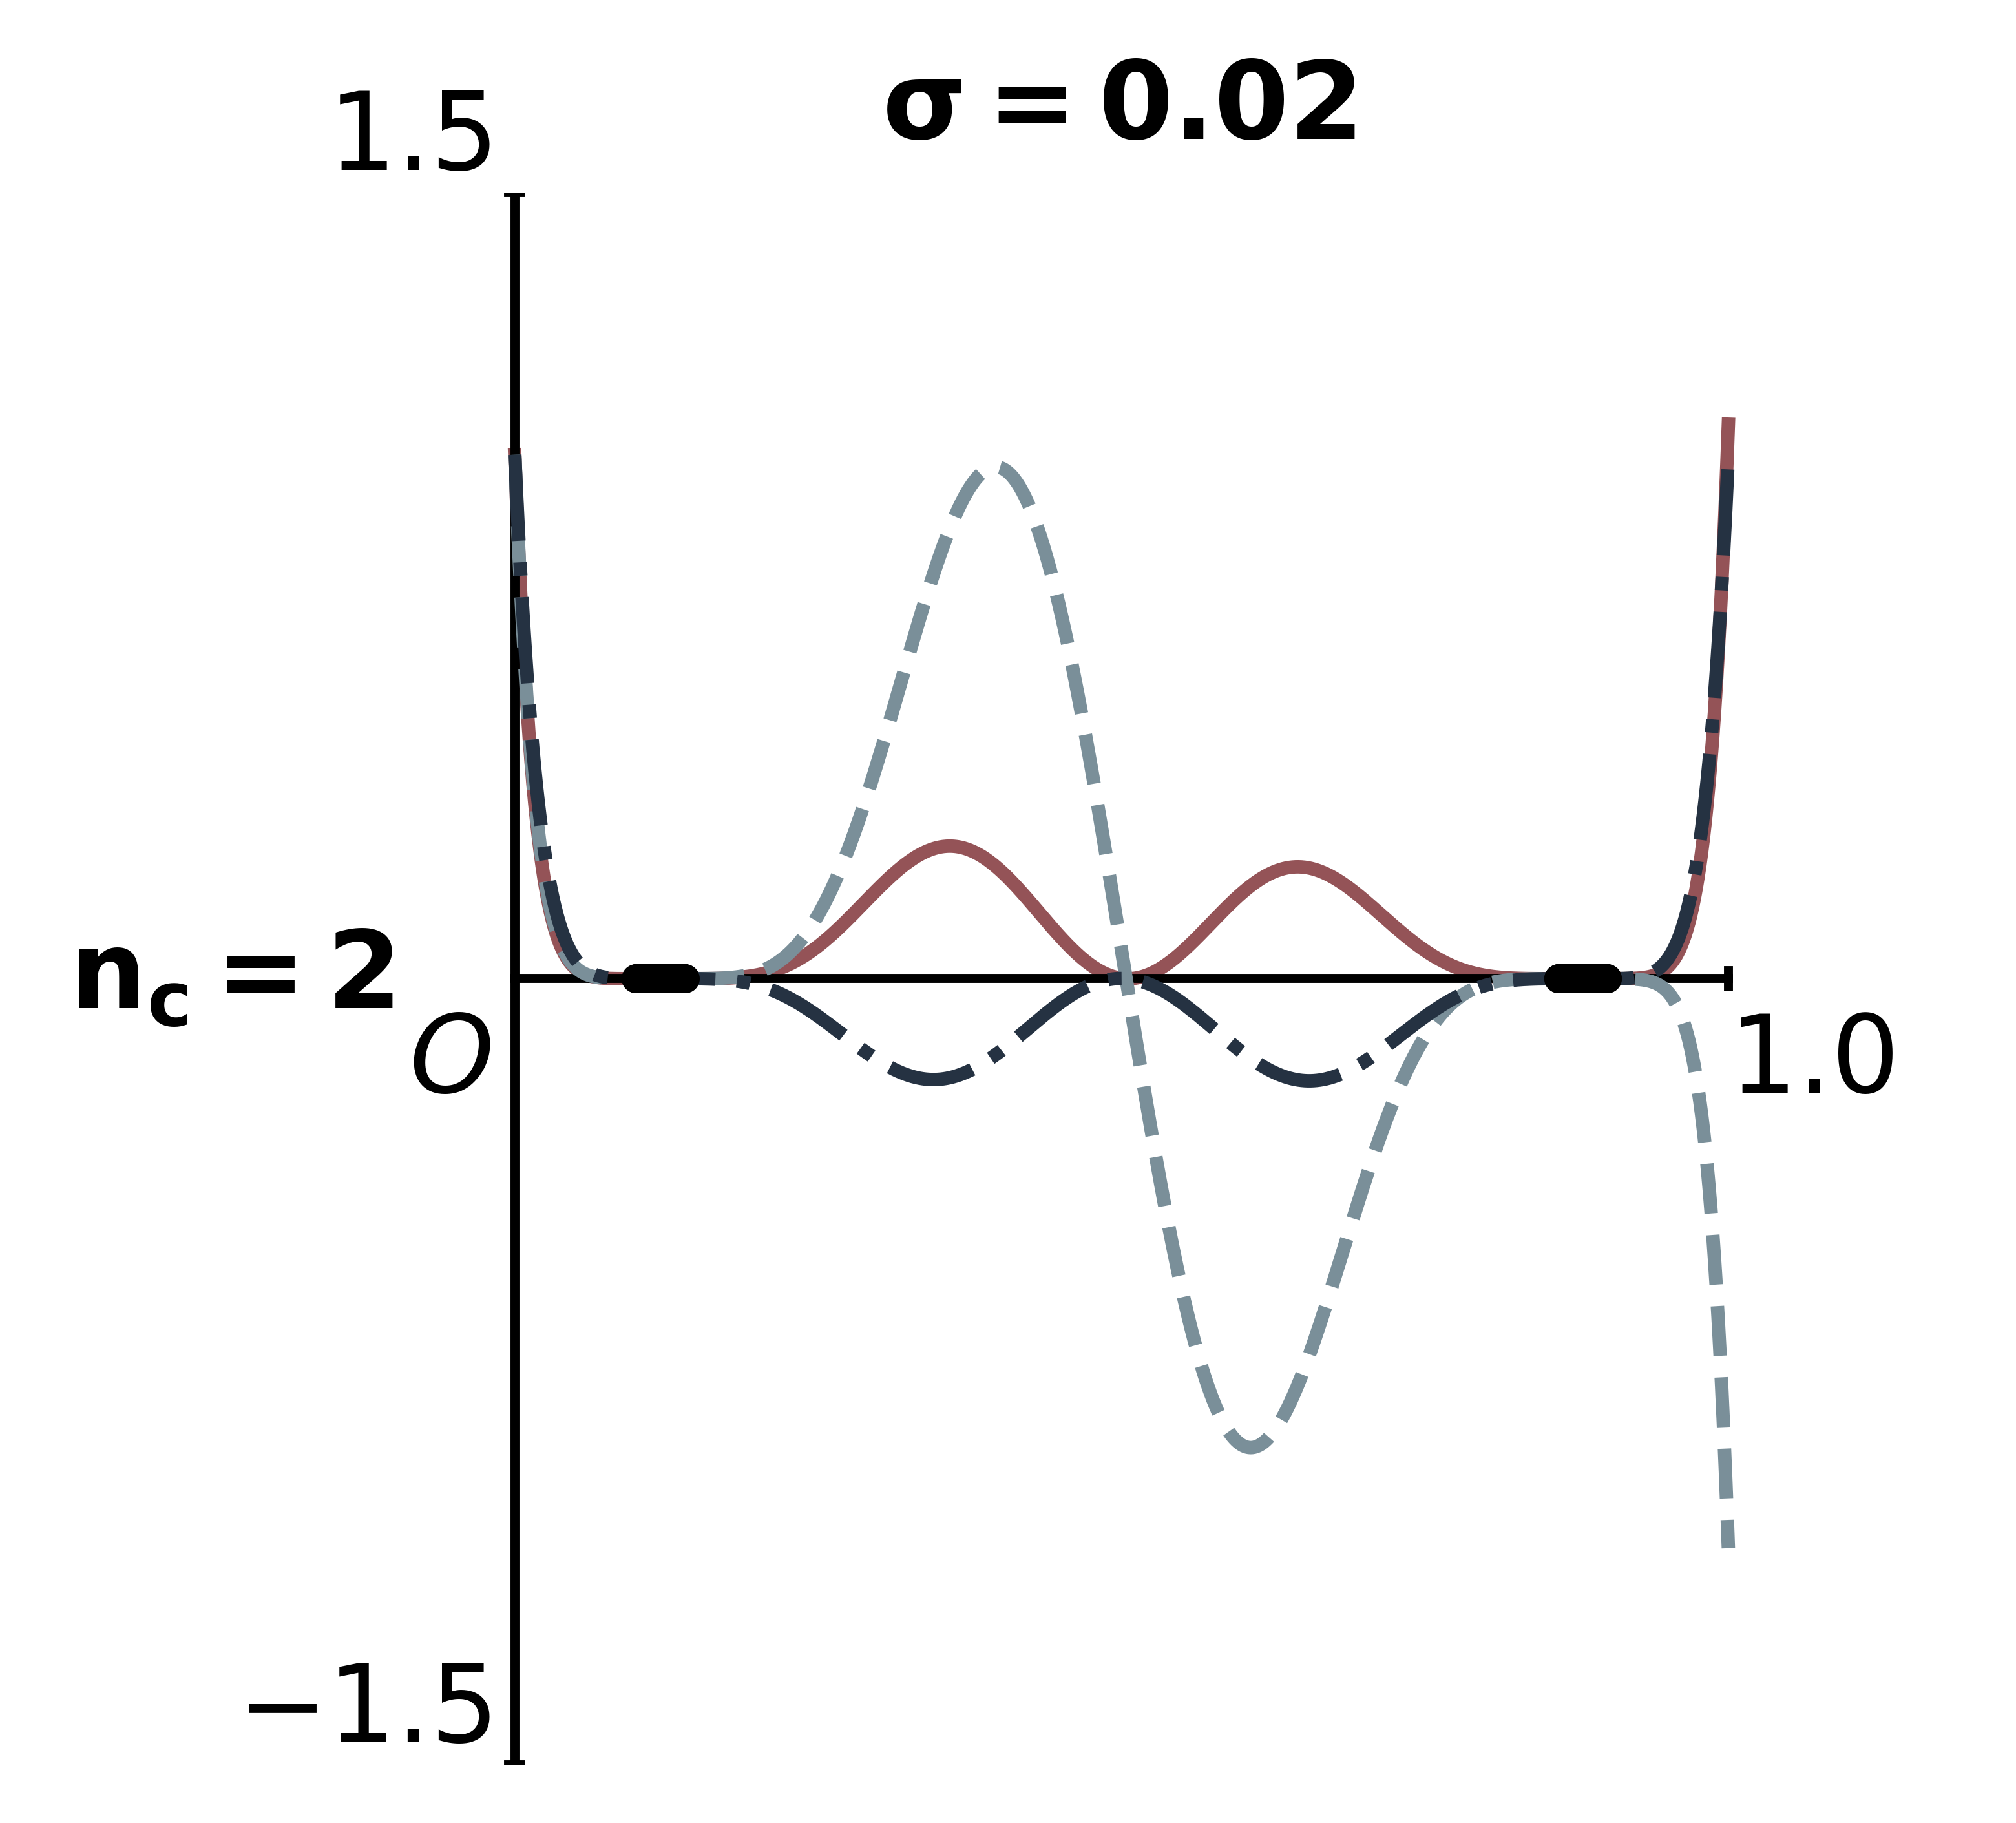
\includegraphics[width=0.8\textwidth]{two_cluster_respoly.png}
                    \caption{Residual polynomial $r_m(\lambda) = 1 - \lambda \alert<3>{q_{m-1}}(\lambda)$}
                \end{figure}
            }
        \end{column}
    \end{columns}
\end{frame}

\begin{frame}[label=background,fragile]
    \frametitle{Mathematical Background}
    \framesubtitle{Conjugate gradient method}
    \begin{itemize}
        \item<1-> Classical (condition number) convergence bound:
        \begin{theorem}
            The error of the $m^{\text{th}}$ iterate of the CG algorithm is bounded by
            \begin{equation*}
            ||\mathbf{e}_m|| \leq 2 \left(\frac{\sqrt{\kappa}-1}{\sqrt{\kappa} + 1}\right)^m ||\mathbf{e}_0||_A,
            \end{equation*}
            where $\kappa = \lambda_{\text{max}}/\lambda_{\text{min}}$ is the condition number of (symmetric matrix) $A$.
        \end{theorem}
        \item<2-> Only sharp for \alert<2>{uniform} eigenvalue distributions!
        \begin{equation*}
            ||\mathbf{e}_m||_A \leq \min_{r \in \mathcal{P}_{m-1}, r(0) = 1} \max_{\lambda \in [\lambda_{\text{min}}, \lambda_{\text{max}}]} |r(\lambda)| ||\mathbf{e}_0||_A \overset{\alert<2>{\text{uniform } \sigma(A)}}{=} \frac{\|\mathbf{e}_0\|}{C_m\left(\frac{\kappa + 1}{\kappa - 1}\right)}
        \end{equation*}
    \end{itemize}
\end{frame}

\begin{frame}[label=background,fragile]
    \frametitle{Mathematical Background}
    \framesubtitle{Conjugate gradient method}
    Setting $\lambda_{\text{min}} = 0.1$ and $\lambda_{\text{max}} = 0.9$ gives $m_{\text{classical}} = 26$. \only<1>{\textcolor{tud grapefruit}{Worst case}}\only<2>{\textcolor{tud green}{Best case}} distribution:
    \only<1>{%
        \begin{figure}
            \centering
            \includegraphics[width=0.7\textwidth]{cg_convergence_extreme_spectra_cluster1.pdf}
            \caption{CG convergence for uniform spectrum.}
        \end{figure}
    }
    \only<2>{%
        \begin{figure}
            \centering
            \includegraphics[width=0.7\textwidth]{cg_convergence_extreme_spectra_cluster0.pdf}
            \caption{CG convergence for spectrum with two distinct eigenvalues.}
        \end{figure}
    }
\end{frame}

% Optimality in the $A$-norm
%             \begin{equation*}
%                 ||\mathbf{e}_m||_A^2 = \min_{r \in \mathcal{P}_{m}, r(0) = 1} \sum_{i=1}^n \frac{r(\lambda_i)^2}{\lambda_i} \mathbf{\rho}_{0,i}^2
%             \end{equation*}

\begin{frame}[label=background,fragile]{Background: Schwarz}
    \frametitle{Mathematical Background}
    \framesubtitle{Schwarz preconditioners}

\end{frame}